\documentclass{beamer}
\usepackage{geometry}
\geometry{paperwidth=21cm,paperheight=7cm}
\setbeamertemplate{navigation symbols}{}
\usepackage{ragged2e}
%\usepackage{fourier}
\usepackage{tikz} 
\usetikzlibrary{chains,shapes.arrows,fit}


\pgfdeclarelayer{background}
\pgfsetlayers{background,main}

\newcounter{task}

\newlength\taskwidth% width of the box for the task description
\newlength\taskvsep% vertical distance between the task description and arrow

\setlength\taskwidth{2.5cm}
\setlength\taskvsep{17pt}

\def\taskpos{}
\def\taskanchor{}

\newcommand\task[1]{%
	{\parbox[t]{\taskwidth}{\scriptsize\Centering#1}}}

\tikzset{
	inner/.style={
		on chain,
		circle,
		inner sep=5pt,
		fill=circlecolor,
		line width=1.7pt,
		draw=bordercolor,
		text width=1.6em,
		align=center,
		text height=1.25ex,
		text depth=0ex
	},
	on grid
}

\newcommand\Task[2][]{%
	\node[inner xsep=0pt] (c1) {\phantom{A}};
	\stepcounter{task}
	\ifodd\thetask\relax
	\renewcommand\taskpos{\taskvsep}\renewcommand\taskanchor{south}
	\else
	\renewcommand\taskpos{-\taskvsep}\renewcommand\taskanchor{north}
	\fi
	\node[inner,font=\footnotesize\sffamily\color{textcolor}]    
	(c\the\numexpr\value{task}+1\relax) {#1};
	\node[anchor=\taskanchor,yshift=\taskpos] 
	at (c\the\numexpr\value{task}+1\relax) {\task{#2}};
}

\newcommand\drawarrow{% the arrow is placed in the background layer 
	% after the node for the tasks have been placed
	\ifnum\thetask=0\relax
	\node[on chain] (c1) {}; % if no \Task command is used, the arrow will be drawn
	\fi
	\node[on chain] (f) {};
	\begin{pgfonlayer}{background}
		\node[
		inner sep=10pt,
		single arrow,
		single arrow head extend=0.8cm,
		draw=none,
		fill=arrowcolor,
		fit= (c1) (f)
		] (arrow) {};
		\fill[white] % the decoration at the tail of the arrow
		(arrow.before tail) -- (c1|-arrow.west) -- (arrow.after tail) -- cycle;
	\end{pgfonlayer}
}

\newenvironment{timeline}[1][node distance=.75\taskwidth]
{\par\noindent\begin{tikzpicture}[start chain,#1]}
	{\drawarrow\end{tikzpicture}\par}
	
	%%%%%%%%%%%%%%%%%%%%%%%%%%%%%%%%%%%%%%%%%%%%%%%%%%%%%%%%%%%%%%%%%%%%%%%%%%%%%%%%%%%%%%%%%%%%%%%%%%%%%%%%%%%%%%%%%%%%%%%%%%%%%%%%%%%%%%%%%%%%%%%%%%%%%%%%%%%%%%%%%%%%%%%%
	\usetikzlibrary{decorations.markings,fadings,shadings}
	\tikzset{pics/blurred arrow/.style={code={
				\tikzset{blurring/.cd,#1}
				\begin{pgfinterruptpicture}%
					\begin{tikzfadingfrompicture}[name=fade right] 
						\shade[left color=transparent!0,
						right color=transparent!100] 
						(0,-\pgfkeysvalueof{/tikz/blurring/line width}) rectangle 
						(\pgfkeysvalueof{/tikz/blurring/length}+\pgfkeysvalueof{/tikz/blurring/line width},\pgfkeysvalueof{/tikz/blurring/line width}); 
					\end{tikzfadingfrompicture}%
				\end{pgfinterruptpicture}
				\newcommand{\bkv}[1]{\pgfkeysvalueof{/tikz/blurring/##1}}
				\begin{scope}[local bounding box=faded]
					% this is the main routine. it draws little rectangles along the upper 
					% and lower border of the path. The size of these rectangles decreases.
					% The decrease is exponential and depends on the drop factor, larger
					% values imply faster decrease (initially it is 0.006).
					\draw[myarrowcolor,line width=\bkv{line width},postaction={decorate,decoration={markings,
							mark=between positions 0 and 1 step 1pt with {
								\pgfmathsetmacro{\myamp}{exp(-(\pgfkeysvalueof{/pgf/decoration/mark info/sequence number}*\bkv{drop factor}))}
								\pgfmathsetmacro{\myoldamp}{exp(-((\pgfkeysvalueof{/pgf/decoration/mark info/sequence number}-1)*\bkv{drop factor}))}
								\shade[top color=white,bottom color=myarrowcolor] 
								(0pt,0.49*\bkv{line width}-\myoldamp*\bkv{amplitude}) 
								-- (0pt,0.49*\bkv{line width}+\myoldamp*\bkv{amplitude}) 
								-- (1.1pt,0.49*\bkv{line width}+\myamp*\bkv{amplitude}) 
								-- (1.1pt,0.49*\bkv{line width}-\myamp*\bkv{amplitude});
								\shade[top color=myarrowcolor,bottom color=white] 
								(0pt,-0.49*\bkv{line width}+\myoldamp*\bkv{amplitude}) 
								-- (0pt,-0.49*\bkv{line width}-\myoldamp*\bkv{amplitude}) 
								-- (1.1pt,-0.49*\bkv{line width}-\myamp*\bkv{amplitude}) 
								-- (1.1pt,-0.49*\bkv{line width}+\myamp*\bkv{amplitude});}}}] 
					(0,0) -- (\bkv{length}, 0);
					% the parts left of the arrow are patched together  
					% left      
					\shade[left color=white,right color=myarrowcolor] 
					(-3*\bkv{amplitude},-0.5*\bkv{line width}+\bkv{amplitude})
					rectangle (0,0.5*\bkv{line width}-\bkv{amplitude});
					% top left  
					\shade[upper left=white,upper right=white,lower left=white,lower right=myarrowcolor] 
					(-3*\bkv{amplitude},0.5*\bkv{line width}-\bkv{amplitude})
					rectangle (0,0.5*\bkv{line width}+\bkv{amplitude});
					% bottom left  
					\shade[upper left=white,upper right=myarrowcolor,lower left=white,lower right=white] 
					(-3*\bkv{amplitude},-0.5*\bkv{line width}+\bkv{amplitude})
					rectangle (0,-0.5*\bkv{line width}-\bkv{amplitude}); 
					%
					\fill[myarrowcolor] (\bkv{length}-\bkv{line width},-\bkv{line width}) 
					-- (\bkv{length}-\bkv{line width},\bkv{line width}) 
					-- (\bkv{length}+\bkv{line width}, 0) -- cycle;
					%
					\pgfmathtruncatemacro{\imax}{-1+\bkv{length}/1cm}
					\foreach \XX in {1,...,\imax}
					{\ifodd\XX
						\draw[myarrowcolor, ultra thick] (\XX*1cm+\pgflinewidth/2-1cm,0) 
						-- (\XX*1cm+\pgflinewidth/2-1cm,\bkv{tick prominence}) 
						node [black, above] {Event \XX};
						\else
						\draw[myarrowcolor, ultra thick] (\XX*1cm+\pgflinewidth/2-1cm,0) 
						-- (\XX*1cm+\pgflinewidth/2-1cm,-\bkv{tick prominence}) 
						node [black, below] {Event \XX};
						\fi
					}
				\end{scope}
				\fill[white,path fading=fade right] (faded.south west) rectangle
				(faded.north east);   
		}},blurring/.cd,amplitude/.initial=2mm,drop factor/.initial=0.006,line
		width/.initial=1cm,%<-width of the arrow line
		length/.initial=9cm,%<- length of the arrow
		tick prominence/.initial=0.8cm,%<- length of the ticks
		color/.code={\colorlet{myarrowcolor}{#1}},
		color=gray}%
		
		
		%%%%%%%%%%%%%%%%%%%%%%%%%%%%%%%%%%%%%%%%%%%%%%%%%%%%%%%%%%%%%%%%%%%%%%%%%%%%%%%%%%%%%%%%%%%%%%%%%%%%%%%%%%%%%%%%%%%%%%%%%%%%%%%%%%%%%%%%%%%%%%%%%%%%%%%%%%%%%%%%%%%%%%%%%%%%%
		\usetikzlibrary{overlay-beamer-styles}
		\tikzset{
			highlight on/.style={alt={#1{fill=red!80!black,color=red!80!black}{fill=gray!30!white,color=gray!30!white}}},
		}
		
		\usepackage{multicol}
		%%%%%%%%%%%%%%%%%%%%%%%%%%%%%%%%%%%%%%%%%%%%%%%%%%%%%%%%%%%%%%%%%%%%%%%%%%%%%%%%%%%%%%%%%%%%%%%%%%%%%%%%%%%%%%%%%%%%%%%%%%%%%%%
\usepackage[utf8]{inputenc}

%\usepackage{geometry}
%\geometry{paperwidth=20cm,paperheight=8cm}

\usepackage{xcolor}
\definecolor{light_red}{RGB}{209,105,81}
\definecolor{light_green}{RGB}{58,181,75}
\definecolor{light_blue}{RGB}{0,153,228}

%\setbeamertemplate{frametitle}[default][center]
\setbeamerfont{footline}{series=\bfseries}
%\setbeamertemplate{footline}[page number]

\usepackage{tikz}
\newcommand{\topline}{%
	\tikz[remember picture, overlay] {%
		\draw[gray, thick] ([xshift = 1cm, yshift = -1.2cm]current page.north west) -- ([xshift = -1cm, yshift = -1.2cm, xshift = \paperwidth]current page.north west);}}
	%%%%%%%%%%%%%%%%%%%%%%%%%%%%%%%%%%%%%%%%%%%%%%%%%%%%%%%%%%%%%%%%%%%%%%%%%%%%%%%%%%%%%%%%%%%%%%%%%%%%%%%%%%%%%%%%%%%%%%%%%%%%%%%%%%%%%%%%%%%%%%%%%%
\usetikzlibrary{calc, arrows.meta, intersections, patterns, positioning, shapes.misc, fadings, through,decorations.pathreplacing}

%\definecolor{ColorOne}{named}{MidnightBlue}
%\definecolor{ColorTwo}{named}{Dandelion}
%\definecolor{ColorThree}{named}{Plum}
%%%%%%%%%%%%%%%%%%%%%%%%%%%%%%%%%%%%%%%%%%%%%%%%%%%%%%%%%%%%%%%%%%%%%%%%%%%%%%%%%%%%%%%%%%%%%%%%%%%%%%%%%%%%%%%
\begin{document}
		\begin{frame}[c]
		\definecolor{arrowcolor}{RGB}{144,168,65}
		\colorlet{circlecolor}{white}
		\definecolor{bordercolor}{RGB}{168,89,65}
		\colorlet{textcolor}{bordercolor}
		%\setlength\taskwidth{1.7cm}
		
		\begin{timeline}
			\Task[Year 1]{Event 1}
			\Task[Year 2]{Event 2}
			\Task[Year 3]{Event 3}
			\Task[Year 4]{Event 4}
			\Task[Year 5]{Event 5}
			\Task[Year 6]{Event 6}
			\Task[Year 7]{Event 7}
			\Task[Year 8]{Event 8}
			\Task[Year 9]{Event 9}
		\end{timeline}
\end{frame}


%%%%%%%%%%%%%%%%%%%%%%%%%%%%%%%%%%%%%%%%%%%%%%%%%%%%%%%%%%%%%%%%%%%%%%%%%%%%
\begin{frame}[c]
	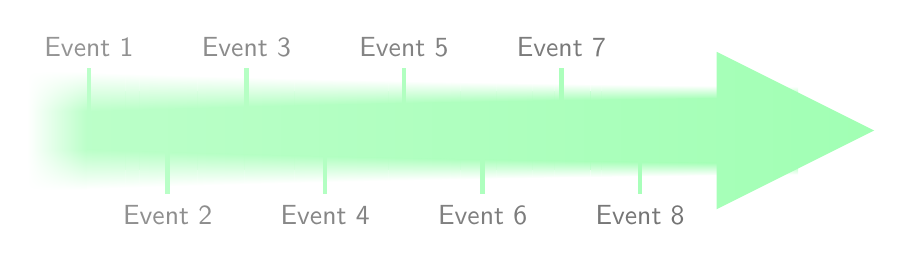
\begin{tikzpicture}[font=\sffamily]
	\pic{blurred arrow={color=lime!50!cyan,amplitude=2.5mm,drop factor=0.005}};
\end{tikzpicture}
\end{frame}


%%%%%%%%%%%%%%%%%%%%%%%%%%%%%%%%%%%%%%%%%%%%%%%%%%%%%%%%%%%%%%%%%%%%%%%%%%%%%

\begin{frame}[c]

\tikzstyle{descript} = [text = black,align=center, minimum height=1.25cm, align=center, outer sep=0pt,font = \footnotesize]
\tikzstyle{activity} =[align=center,outer sep=1pt]

\begin{tikzpicture}[very thick, black]
	
	%% Coordinates
	\coordinate (O) at (-3,0); % Origin
	\coordinate (P1) at (3,0);
	\coordinate (P2) at (7,0);
	\coordinate (P3) at (11,0);
	\coordinate (F) at (15,0); %End
	\coordinate (E1) at (4,0); %Event
	\coordinate (E2) at (-0.5,0); %Event
	\coordinate (X0) at (-1,0);
	\coordinate (X1) at (3,0);
	\coordinate (X2) at (6,0);
	\coordinate (X3) at (7,0);
	\coordinate (X4) at (10,0);
	
	
	%% Filled regions
	%\fill[color=ColorOne!20] rectangle (O) -- (X0) -- ($(X0)+(0,1)$) -- ($(O)+(0,1)$); % Studies
	\shade[right color=black!50, left color=white] rectangle (O) -- (X0) -- ($(X0)+(0,1)$) -- ($(O)+(0,1)$); % Current work
	\fill[color=violet!50] rectangle (X0) -- (X1) -- ($(X1)+(0,1)$) -- ($(X0)+(0,1)$); %
	\fill[color=blue!50] rectangle (X1) -- (X2) -- ($(X2)+(0,1)$) -- ($(X1)+(0,1)$); % 
	\fill[color=cyan!50] rectangle (X2) -- (X3) -- ($(X3)+(0,1)$) -- ($(X2)+(0,1)$); % Work
	\fill[color=red!50] rectangle (X3) -- (X4) -- ($(X4)+(0,1)$) -- ($(X3)+(0,1)$); % Work
	\fill[color=yellow!50] rectangle (X4) -- (P3) -- ($(P3)+(0,1)$) -- ($(X4)+(0,1)$); % Work
	\shade[left color=green, right color=white] rectangle (P3) -- (F) -- ($(F)+(0,1)$) -- ($(P3)+(0,1)$); % Current work
	
	\path [pattern color=red, pattern=north east lines, line width = 1pt, very thick] rectangle ($(X0)+(0,0)$) -- ($(X0)+(0.0,0)$) -- ($(X0)+(-0.5,1)$) -- ($(X0)+(0.5,1)$); % Something else
	\path [pattern color=black, pattern=north east lines, line width = 1pt, very thick] rectangle ($(X1)+(0.0,0)$) -- ($(X1)+(0.0,0)$) -- ($(X1)+(-0.5,1)$) -- ($(X1)+(0.5,1)$); % Something else
	\path [pattern color=yellow, pattern=north east lines, line width = 1pt, very thick] rectangle ($(X2)+(0.0,0)$) -- ($(X2)+(0.0,0)$) -- ($(X2)+(-0.5,1)$) -- ($(X2)+(0.5,1)$); % Something else		
	\path [pattern color=blue, pattern=north east lines, line width = 1pt, very thick] rectangle ($(X3)+(0.0,0)$) -- ($(X3)+(0.0,0)$) -- ($(X3)+(-0.5,1)$) -- ($(X3)+(0.5,1)$); % Something else		
	\path [pattern color=magenta, pattern=north east lines, line width = 1pt, very thick] rectangle ($(X4)+(0.0,0)$) -- ($(X4)+(0.0,0)$) -- ($(X4)+(-0.5,1)$) -- ($(X4)+(0.5,1)$); % Something else		
	\path [pattern color=violet!50!green, pattern=north east lines, line width = 1pt, very thick] rectangle ($(P3)+(0.0,0)$) -- ($(P3)+(0.0,0)$) -- ($(P3)+(-0.5,1)$) -- ($(P3)+(0.5,1)$); % Something else	
	
	%% Description
	\node[descript,fill=red!15,text=black](D0) at ($(X0)+(-2,-2.5)$) {TEXT red};
	
	\node[descript,fill=gray!60,text=black](D2) at ($(X1)+(-4,3)$) {TEXT gray};
	
	\node[descript,fill=yellow!60,text=black](D3) at ($(X2)+(-4,-2.5)$) {TEXT yellow};
	
	\node[descript,fill=blue!15,text=black](D4) at ($(X3)+(-4.8,3)$) {TEXT blue};		
	
	\node[descript,fill=green!20,text=black](D5) at ($(X4)+(-3,-2.5)$) {TEXT Green};
	
	\node[descript,fill=magenta!40,text=black](D6) at ($(P3)+(-2.2,3)$){TEXT Mgenta};
	
	\node[descript,fill=orange!25,text=black](D7) at ($(P3)+(2,-2.5)$) {TEXT Orange};
	
	\node[descript,fill=violet!25,text=black](D8) at ($(P3)+(3,3)$) {TEXT Purple};		
	
	%% Arrows
	\path[->,color=red, line width=1.5mm] ($(X0)$) edge [out=-50, in=90]  ($(D0)+(0,1)$);
	\path[->,color=black, line width=1.5mm] ($(X1)$) edge [out=70, in=-130]  ($(D2)+(0,-1)$);
	\path[->,color=yellow!70!black, line width=1.5mm]($(X2)$)  edge [out=-50, in=90]  ($(D3)+(0,1)$);
	\path[->,color=blue, line width=1.5mm]($(X3)$)  edge [out=100, in=-90]  ($(D4)+(0,-1)$);	
	\path[->,color=green, line width=1.5mm]($(X4)$)  edge [out=-70, in=90]  ($(D5)+(0,1)$);	
	\path[->,color=magenta, line width=1.5mm]($(P3)$)  edge [out=70, in=-90]  ($(D6)+(0,-1)$);
	\path[->,color=orange, line width=1.5mm]($(P3)$)  edge [out=-70, in=90]  ($(D7)+(0,1)$);	
	\path[->,color=violet, line width=1.5mm]($(P3)$)  edge [out=70, in=-90]  ($(D8)+(0,-1)$);	
	
	%% Arrow
	\draw[->>, pattern=crosshatch, line width=1.5mm] ($(O)+(0,0.2)$) -- ($(F)+(0,0.2)$);
	%% Ticks
	\foreach \x in {-4,-3,...,17}
	\draw(\x cm,6pt) -- (\x cm,0pt);
	%% Labels
	\foreach \i \j in {0/\textbf{\large Yr 1},3/\textbf{\large Yr 2},7/\textbf{\large Yr 3},9/\textbf{\large Yr 4},11/\textbf{\large Yr 5},12.1/\textbf{\large Yr 6},13.5/\textbf{\large Yr 7}}{
		\draw (\i,0) node[below=3pt] {\j} ;
	}
	
\end{tikzpicture}
\end{frame}

%%%%%%%%%%%%%%%%%%%%%%%%%%%%%%%%%%%%%%%%%%%%%%%%%%%%%%%%%%%%%%%%%%%%%%%%%%%%%
\begin{frame}[c]
	%\frametitle{\color{light_red}\textbf{Background}}
%	\topline

\noindent\rule[1ex]{\linewidth}{5pt}
\textbf{Chaos Theory}
\noindent\rule[0ex]{\linewidth}{0.2pt}
\resizebox{18cm}{!}{
	\begin{tikzpicture}
		
		%%% B. F. Skinner %%%
		\pgfdeclareimage[height = 4cm]{aristotle}{Aristotle.jpg}
		\node (aristotle) at (0, 0) {\pgfuseimage{aristotle}};
		\draw (0, 2.5) node {\color{light_red}\textbf{ABC}};
		\draw (0, -2.5) node {\large\textbf{Aristotle}};
		
		\node [circle, line width = 1mm, draw = light_blue, fill = green, minimum size = 0.4cm] (node1) at (0, 3.2) {};
		\draw (0, 4) node {\Large\textbf{350 BCE}};
		
		%%% Social Learning book 1 %%%
		\node [circle, line width = 1mm, draw = red, fill = red, minimum size = 0.4cm] (node2) at (5, 3.2) {};
		
		\pgfdeclareimage[height = 4cm]{poincaré}{Henri_Poincaré-2.jpg}
		\node (poincaré) at (5, 0) {\pgfuseimage{poincaré}};
		\draw (5, 4) node {\Large\textbf{1890}};
		\draw (5, 2.7) node {\color{light_red}\textbf{\large{Three-Body}}};
		\draw (5, 2.3) node {\color{light_red}\textbf{\large{Problem}}};
		\draw (5, -2.5) node {\large\textbf{Henri Poincaré}};
		%\draw (5, 0.8) node {\large\textbf{John Dollard}};
		
		%%% Path Aristotle and poincaré %%%
		%\path [line width = 1mm, draw = light_blue, -] (node1) edge (node2);
		
		%%% Social Learning book 2 %%%
		\node [circle, line width = 1mm, draw = light_blue, fill = white, minimum size = 0.4cm] (node3) at (10, 3.2) {};
		
		\pgfdeclareimage[height = 4cm]{hadamard}{Hadamard2.jpg}
		\node (hadamard) at (10, 0) {\pgfuseimage{hadamard}};
		\draw (10, 4) node {\Large\textbf{1898}};
		\draw (10, 2.7) node {\color{light_red}\textbf{\large{Motion  on certain}}};
		\draw (10, 2.3) node {\color{light_red}\textbf{\large{  surfaces always diverge}}};
		\draw (10, -2.5) node {\large\textbf{Jacques Hadamard}};
		
		%%% Path between book 1 and book 2 %%%
		\draw [line width = 1mm, draw = light_blue]  (5.2, 3.2) -- (7.5, 3.2) -- (7.6, 3.5) -- (7.8, 2.9) -- (7.9, 3.2) -- (9.8, 3.2);
		
		%%% Noam Chomsky %%%
		\pgfdeclareimage[height = 4cm]{cartwright}{cartwright}
		\node (cartwright) at (15, 0) {\pgfuseimage{cartwright}};
		\node [circle, line width = 1mm, draw = light_blue, fill = white, minimum size = 0.4cm] (node4) at (15, 3.2) {};
		\draw (15, 4) node {\Large\textbf{1931}};
		\draw (15, 2.7) node {\color{light_red}\textbf{\large{ Studied Van der Pol}}};
		\draw (15, 2.3) node {\color{light_red}\textbf{\large{equation}}};
		\draw (15, -2.5) node {\large\textbf{Mary Lucy Cartwright}};
		
		%%% Path between book 2 and Chomsky %%%
		\draw [line width = 1mm, draw = light_blue]  (5.2 + 5, 3.2) -- (7.5 + 5, 3.2) -- (7.6 + 5, 3.5) -- (7.8 + 5, 2.9) -- (7.9 + 5, 3.2) -- (9.8 + 5, 3.2);
		
		%%% Albert Bandura %%%
		\pgfdeclareimage[height = 4cm]{lorenz}{lorenz.jpg}	\node (lorenz) at (20, 0) {\pgfuseimage{lorenz}};
		\node [circle, line width = 1mm, draw = red, fill = red, minimum size = 0.4cm] (node5) at (20, 3.2) {};
		\draw (20, 4) node {\Large\textbf{1963}};
		\draw (20, 2.7) node {\color{light_red}\textbf{\large{Butterfly}}};
		\draw (20, 2.3) node {\color{light_red}\textbf{\large{Effect}}};
		\draw (20, -2.5) node {\large\textbf{Edward Norton Lorenz }};
		
		%%% Path between Chomsky and Bandura %%%
		\draw [line width = 1mm, draw = light_blue]  (5.2 + 10, 3.2) -- (7.5 + 10, 3.2) -- (7.6 + 10, 3.5) -- (7.8 + 10, 2.9) -- (7.9 + 10, 3.2) -- (9.8 + 10, 3.2);
		
		%%% RichardMiller %%%
		\pgfdeclareimage[width= 5cm]{RichardMiller}{RichardMiller.jpg}	
		\node (RichardMiller) at (25, 0) {\pgfuseimage{RichardMiller}};
		\node [circle, line width = 1mm, draw = light_blue, fill = white, minimum size = 0.4cm] (node5) at (25, 3.2) {};
		\draw (25, 4) node {\Large\textbf{1964}};
		\draw (25, 2.7) node {\color{light_red}\textbf{\large{First demonstration of the}}};
		\draw (25, 2.3) node {\color{light_red}\textbf{\large{ exponential divergence of}}};
		\draw (25, 1.9) node {\color{light_red}\textbf{\large{	chaotic trajectories}}};
		\draw (25, -2.5) node {\large\textbf{ Richard H. Miller}};	
		
		\draw [line width = 1mm, draw = light_blue]  (5.2 + 15, 3.2) --  (9.8 + 15, 3.2);
		
		%%% Mandelbrot %%%
		\pgfdeclareimage[height = 4cm]{Mandelbrot}{Mandelbrot.jpg}	\node (Mandelbrot) at (30, 0) {\pgfuseimage{Mandelbrot}};
		\node [circle, line width = 1mm, draw = light_blue, fill = white, minimum size = 0.4cm] (node5) at (30, 3.2) {};
		\draw (30, 4) node {\Large\textbf{1967}};
		\draw (30, 2.7) node {\color{light_red}\textbf{\large{Mandelbrot}}};
		\draw (30, 2.3) node {\color{light_red}\textbf{\large{Set}}};
		\draw (30, -2.5) node {\large\textbf{ Benoit Mandelbrot}};			
		
		\draw [line width = 1mm, draw = light_blue]  (5.2 + 20, 3.2) --  (9.8 + 20, 3.2);
		
		%%% Gutzwiller %%%
		\pgfdeclareimage[height = 4cm]{MGutzwiller}{gutzwiller.jpg}	
		\node (MGutzwiller) at (35, 0) {\pgfuseimage{MGutzwiller}};
		\node [circle, line width = 1mm, draw = light_green, fill = white, minimum size = 0.4cm] (node5) at (35, 3.2) {};
		\draw (35, 4) node {\Large\textbf{1971}};
		\draw (35, 2.7) node {\color{light_red}\textbf{\large{Gutzwiller}}};
		\draw (35, 2.3) node {\color{light_red}\textbf{\large{Trace Formula}}};
		\draw (35, -2.5) node {\large\textbf{M. C. Gutzwiller}};	
		
		\draw [line width = 1mm, draw = light_blue]  (5.2 + 25, 3.2) -- (7.5 + 25, 3.2) -- (7.6 + 25, 3.5) -- (7.8 + 25, 2.9) -- (7.9 + 25, 3.2) -- (9.8 + 25, 3.2);
		
		%Ruelle_Takens
		\pgfdeclareimage[width= 5cm]{Ruelle_Takens}{Ruelle_Takens.jpg}	
		\node (MGutzwiller) at (40, 0) {\pgfuseimage{Ruelle_Takens}};
		\node [circle, line width = 1mm, draw = light_green, fill = white, minimum size = 0.4cm] (node5) at (40, 3.2) {};
		\draw (40, 4) node {\Large\textbf{1971}};
		\draw (40, 2.7) node {\color{light_red}\textbf{\large{Strange}}};
		\draw (40, 2.3) node {\color{light_red}\textbf{\large{Attractor}}};
		\draw (40, -2.0) node {\large\textbf{ David Ruelle \& Floris Takens}};
		\draw (40, -2.5) node {\large\textbf{\& Floris Takens}};
		
		\draw [line width = 1mm, draw = green, dashed]  (5.2 + 30, 3.2) --  (9.8 + 30, 3.2);
		
		%%% Feigenbaum%%%
		\pgfdeclareimage[height = 4cm]{Feigenbaum}{Feigenbaum.jpg}	\node (Feigenbaum) at (45, 0) {\pgfuseimage{Feigenbaum}};
		\node [circle, line width = 1mm, draw = light_blue, fill = white, minimum size = 0.4cm] (node5) at (45, 3.2) {};
		\draw (45, 4) node {\Large\textbf{1975}};
		\draw (45, 2.7) node {\color{light_red}\textbf{\large{Feigenbaum}}};
		\draw (45, 2.3) node {\color{light_red}\textbf{\large{Constant}}};
		\draw (45, -2.5) node {\large\textbf{ Mitchell J. Feigenbaum}};			
		
		\draw [line width = 1mm, draw = light_blue]  (5.2 + 35, 3.2) --  (9.8 + 35, 3.2);
		
		%%% berry-tobar %%%
		\pgfdeclareimage[width = 5cm]{beey_tobar}{beey_tobar.jpg}	\node (beey_tobar) at (50, 0) {\pgfuseimage{beey_tobar}};
		\node [circle, line width = 1mm, draw = light_blue, fill = white, minimum size = 0.4cm] (node5) at (50, 3.2) {};
		\draw (50, 4) node {\Large\textbf{1977}};
		\draw (50, 2.7) node {\color{light_red}\textbf{\large{Berry and Tabor}}};
		\draw (50, 2.3) node {\color{light_red}\textbf{\large{Conjecture}}};
		\draw (50, -2.0) node {\large\textbf{Sir Michael Victor Berry}};	
		\draw (50, -2.5) node {\large\textbf{ \& Michael Tabor}};			
		
		\draw [line width = 1mm, draw = light_blue]  (5.2 + 40, 3.2) --  (9.8 + 40, 3.2);	
		
		%%% kicked rotor %%%
		\pgfdeclareimage[height= 4cm]{qkr}{QKR.jpg}	
		\node (qkr) at (55, 0) {\pgfuseimage{qkr}};
		\node [circle, line width = 1mm, draw = light_blue, fill = white, minimum size = 0.4cm] (node5) at (55, 3.2) {};
		\draw (55, 4) node {\Large\textbf{1979}};
		\draw (55, 2.7) node {\color{light_red}\textbf{\large{Quantum}}};
		\draw (55, 2.3) node {\color{light_red}\textbf{\large{Kicked Rotor}}};
		\draw (55, -2.5) node {\large\textbf{Joseph Ford, Giulio Casati,}};	
		\draw (55, -3.0) node {\large\textbf{ Boris Chirikov, \& Fritz Izrailev}};			
		
		\draw [line width = 1mm, draw = light_blue]  (5.2 + 45, 3.2) --  (9.8 + 45, 3.2);	
		
		
		%%% OriolBohigas %%%
		\pgfdeclareimage[height= 4cm]{OriolBohigas}{OriolBohigas.jpg}	
		\node (OriolBohigas) at (60, 0) {\pgfuseimage{OriolBohigas}};
		\node [circle, line width = 1mm, draw = red, fill = red, minimum size = 0.4cm] (node5) at (60, 3.2) {};
		\draw (60, 4) node {\Large\textbf{1984}};
		\draw (60, 2.7) node {\color{light_red}\textbf{\large{BGS Conjecture}}};
		\draw (60, 2.3) node {\color{light_red}\textbf{\large{Random Matrix Universality}}};
		\draw (60, -2.5) node {\large\textbf{Oriol Bohigas Martí,}};	
		%\draw (52, -2.0) node {\large\textbf{ Marie-Joya Giannoni,}};			
		%\draw (52, -2.5) node {\large\textbf{ Marie-Joya Giannoni,}};			
		
		\draw [line width = 1mm, draw = light_blue]  (5.2 + 50, 3.2) -- (7.5 + 50, 3.2) -- (7.6 + 50, 3.5) -- (7.8 + 50, 2.9) -- (7.9 + 50, 3.2) -- (9.8 + 50, 3.2);
		
		%%% mss bound %%%
		\pgfdeclareimage[width= 5cm]{MSS}{MSS.jpg}	
		\node (MSS) at (65, 0) {\pgfuseimage{MSS}};
		\node [circle, line width = 1mm, draw = red, fill = red, minimum size = 0.4cm] (node5) at (65, 3.2) {};
		\draw (65, 4) node {\Large\textbf{2015}};
		\draw (65, 2.7) node {\color{light_red}\textbf{\large{MSS Bound}}};
		%\draw (65, 2.3) node {\color{light_red}\textbf{\large{Random Matrix Universality}}};
		\draw (65, -1.5) node {\large\textbf{Juan Maldacena,}};	
		\draw (65, -2.0) node {\large\textbf{Stephen H. Shenker,}};			
		\draw (65, -2.5) node {\large\textbf{\& Douglas Stanford}};			
		
		\draw [line width = 1mm, draw = light_blue]  (5.2 + 55, 3.2) -- (7.5 + 55, 3.2) -- (7.6 + 55, 3.5) -- (7.8 + 55, 2.9) -- (7.9 + 55, 3.2) -- (9.8 + 55, 3.2);		
		
		
		%%% Path between Chomsky and Bandura %%%
		\draw [line width = 1mm, draw = light_blue]  (5.2 + 60, 3.2) -- (7.5 + 60, 3.2) -- (7.6 + 60, 3.5) -- (7.8 + 60, 2.9) -- (7.9 + 60, 3.2) -- (9.8 + 60, 3.2);
		
		%%% Path between Chomsky and Bandura %%%
		%\draw [line width = 1mm, draw = light_green]  (5.2 + 65, 3.2) -- (6.5 + 65, 3.2) -- (6.6 + 65, 3.5) -- (6.8 + 65, 2.9) -- (6.9 + 65, 3.2) -- (7.8 + 65, 3.2);
		
	\end{tikzpicture}
}
\noindent\rule[1ex]{\linewidth}{5pt}

\end{frame}

\begin{frame}[c]
	%\frametitle{\color{light_red}\textbf{Background}}
%	\topline

\textbf{Quantum Mechanics}
\noindent\rule[0ex]{\linewidth}{0.2pt}
\resizebox{18cm}{!}{
	\begin{tikzpicture}
		
		%%% B. F. Skinner %%%
		\pgfdeclareimage[height = 4cm]{MaxP}{MaxP}
		\node (MaxP) at (0, -7) {\pgfuseimage{MaxP}};
		\draw (0, -4.3) node {\color{light_red}\textbf{\large{Black Body}}};
		\draw (0, -4.7) node {\color{light_red}\textbf{\large{Radiation}}};
		\draw (0, -9.5) node {\large\textbf{Max Planck}};
		
		\node [circle, line width = 1mm, draw = red, fill = red, minimum size = 0.4cm] (node1) at (0, -3.8) {};
		\draw (0, -3) node {\Large\textbf{1900}};
		
		%%% Social Learning book 1 %%%
		\node [circle, line width = 1mm, draw = red, fill = red, minimum size = 0.4cm] (node2) at (5, -3.8) {};
		
		\pgfdeclareimage[height = 4cm]{einstein}{albert-einstein.jpg}
		\node (einstein) at (5, -7) {\pgfuseimage{einstein}};
		\draw (5, -3) node {\Large\textbf{1905}};
		\draw (5, -4.3) node {\color{light_red}\textbf{\large{Photo Electric}}};
		\draw (5, -4.7) node {\color{light_red}\textbf{\large{Effect}}};
		\draw (5, -9.5) node {\large\textbf{Albert Einstein}};
		
		
		%%% Path between Skinner and Social Learning book 1 %%%
		\path [line width = 1mm, draw = light_blue, -] (node1) edge (node2);
		
		%%% Social Learning book 2 %%%
		\node [circle, line width = 1mm, draw = light_blue, fill = white, minimum size = 0.4cm] (node3) at (10, -3.8) {};
		
		\pgfdeclareimage[height = 4cm]{rutherford}{Rutherford}
		\node (rutherford) at (10, -7) {\pgfuseimage{rutherford}};
		\draw (10, -3) node {\Large\textbf{1911}};
		\draw (10, -4.3) node {\color{light_red}\textbf{\large{Discovery of}}};
		\draw (10, -4.7) node {\color{light_red}\textbf{\large{Nucleus Charge}}};
		\draw (10, -9.5) node {\large\textbf{Ernest Rutherford}};
		
		%%% Path between book 1 and book 2 %%%
		\draw [line width = 1mm, draw = light_blue]  (5.2, -3.8)-- (9.8, -3.8);
		
		%%% Noam Chomsky %%%
		\pgfdeclareimage[height = 4cm]{Bohr}{Bohr}
		\node (Bohr) at (14, -7) {\pgfuseimage{Bohr}};
		\node [circle, line width = 1mm, draw = light_blue, fill = white, minimum size = 0.4cm] (node4) at (14, -3.8) {};
		\draw (14, -3) node {\Large\textbf{1913}};
		\draw (14, -4.3) node {\color{light_red}\textbf{\large{Atomic structure}}};
		\draw (14, -4.7) node {\color{light_red}\textbf{\large{Model}}};
		\draw (14, -9.5) node {\large\textbf{Niels Bohr}};
		
		%%% Path between book 2 and Chomsky %%%
		\draw [line width = 1mm, draw = light_blue]  (5.2 + 5, -3.8) -- (9.8 + 4, -3.8);
		
		%%% Albert Bandura %%%
		\pgfdeclareimage[width = 5cm]{SG}{SG}
		\node (SG) at (19, -7) {\pgfuseimage{SG}};
		\node [circle, line width = 1mm, draw = light_green, fill = white, minimum size = 0.4cm] (node5) at (19, -3.8) {};
		\draw (19, -3) node {\Large\textbf{1922}};
		\draw (19, -4.3) node {\color{light_red}\textbf{\large{Stern-Gerlach}}};
		\draw (19, -4.7) node {\color{light_red}\textbf{\large{ Experiment}}};
		\draw (19, -5.1) node {\color{light_red}\textbf{\large{(Spin quantization)}}};
		\draw (19, -9.5) node {\large\textbf{Otto Stern \&  Walter Gerlach }};
		
		%%% Path between Chomsky and Bandura %%%
		\draw [line width = 1mm, draw = light_blue]  (5.2 + 9, -3.8) -- (7.5 + 9, -3.8) -- (7.6 + 9, -3.5) -- (7.8 + 9, -4.1) -- (7.9 + 9, -3.8) -- (9.8 + 9, -3.8);
		
		
		%1924
		\pgfdeclareimage[height = 4cm]{broglie}{Broglie}
		\node (SG) at (24, -7) {\pgfuseimage{broglie}};
		\node [circle, line width = 1mm, draw = red, fill = red, minimum size = 0.4cm] (node5) at (24, -3.8) {};
		\draw (24, -3) node {\Large\textbf{1924}};
		\draw (24, -4.3) node {\color{light_red}\textbf{\large{Wave-Particle}}};
		\draw (24, -4.7) node {\color{light_red}\textbf{\large{Duality}}};
		\draw (24, -9.5) node {\large\textbf{Louis De Broglie}};	
		
		\draw [line width = 1mm, draw = light_blue]  (5.2 + 14, -3.8) -- (9.8 + 14, -3.8);
		
		%1925
		\pgfdeclareimage[height = 4cm]{pauli}{Pauli}
		\node (pauli) at (28, -7) {\pgfuseimage{pauli}};
		\node [circle, line width = 1mm, draw = red, fill = red, minimum size = 0.4cm] (node5) at (28, -3.8) {};
		\draw (28, -3) node {\Large\textbf{1925}};
		\draw (28, -4.3) node {\color{light_red}\textbf{\large{Introduction of}}};
		\draw (28, -4.7) node {\color{light_red}\textbf{\large{Spin}}};
		\draw (28, -9.5) node {\large\textbf{Wolfgang Pauli}};	
		
		\draw [line width = 1mm, draw = light_blue]  (5.2 + 19, -3.8) -- (9.8 + 18, -3.8);		
		
		%1926		
		\pgfdeclareimage[height = 4cm]{Schrödinger}{Erwin_Schrödinger}
		\node (Schrödinger) at (32, -7) {\pgfuseimage{Schrödinger}};
		\node [circle, line width = 1mm, draw = red, fill = red, minimum size = 0.4cm] (node5) at (32, -3.8) {};
		\draw (32, -3) node {\Large\textbf{1926}};
		\draw (32, -4.3) node {\color{light_red}\textbf{\large{Schrödinger}}};
		\draw (32, -4.7) node {\color{light_red}\textbf{\large{wave Equation}}};
		\draw (32, -9.5) node {\large\textbf{Erwin Schrödinger}};	
		
		\draw [line width = 1mm, draw = light_blue]  (5.2 + 23, -3.8) -- (9.8 + 22, -3.8);		
		
		%1927		
		\pgfdeclareimage[height = 4cm]{Heisenberg}{heisenberg_werner}
		\node (Heisenberg) at (36, -7) {\pgfuseimage{Heisenberg}};
		\node [circle, line width = 1mm, draw = red, fill = red, minimum size = 0.4cm] (node5) at (36, -3.8) {};
		\draw (36, -3) node {\Large\textbf{1927}};
		\draw (36, -4.3) node {\color{light_red}\textbf{\large{ Uncertainty}}};
		\draw (36, -4.7) node {\color{light_red}\textbf{\large{Principle}}};
		\draw (36, -9.5) node {\large\textbf{Werner Heisenberg}};	
		
		\draw [line width = 1mm, draw = light_blue]  (5.2 + 27, -3.8) -- (9.8 + 26, -3.8);
		%-1927
		\pgfdeclareimage[height = 4cm]{Dirac}{Paul_Dirac}
		\node (Dirac) at (40, -7) {\pgfuseimage{Dirac}};
		\node [circle, line width = 1mm, draw = red, fill = red, minimum size = 0.4cm] (node5) at (40, -3.8) {};
		\draw (40, -3) node {\Large\textbf{1927}};
		\draw (40, -4.3) node {\color{light_red}\textbf{\large{ Relativistic }}};
		\draw (40, -4.7) node {\color{light_red}\textbf{\large{Quantum Mechanics}}};
		\draw (40, -9.5) node {\large\textbf{Paul Dirac}};
		
		\draw [line width = 1mm, draw = green, dashed]  (5.2 + 31, -3.8) -- (9.8 + 30, -3.8);
		
		
		%-1927-40s
		\pgfdeclareimage[height = 4cm]{qft}{qft.jpg}
		\node (qft) at (45, -7) {\pgfuseimage{qft}};
		\node [circle, line width = 1mm, draw = light_green, fill = white, minimum size = 0.4cm] (node5) at (45, -3.8) {};
		\draw (45, -3) node {\Large\textbf{1927-1940s}};
		\draw (45, -4.3) node {\color{light_red}\textbf{\large{ Quantum }}};
		\draw (45, -4.7) node {\color{light_red}\textbf{\large{Field Theory}}};
		\draw (45, -9.5) node {\large\textbf{ R.P. Feynman, S. Tomonag}};
		\draw (45, -10) node {\large\textbf{J. Schwinger \& F. Dyson}};
		
		
		\draw [line width = 1mm, draw = light_blue]  (5.2 + 35, -3.8) -- (6.5 + 36, -3.8) -- (6.6 + 36, -3.5) -- (6.8 + 36, -4.1) -- (6.9 + 36, -3.8) --(9.8 + 35, -3.8);
		
		%-1960s-70s
		\pgfdeclareimage[width = 5cm]{qft}{ChromoD.jpg}
		\node (qft) at (50, -7) {\pgfuseimage{qft}};
		\node [circle, line width = 1mm, draw = light_green, fill = white, minimum size = 0.4cm] (node5) at (50, -3.8) {};
		\draw (50, -3) node {\Large\textbf{1960s-1970s}};
		\draw (50, -4.3) node {\color{light_red}\textbf{\large{ Quantum }}};
		\draw (50, -4.7) node {\color{light_red}\textbf{\large{Chromodynamics}}};
		\draw (50, -9.0) node {\large\textbf{David Gross,}};
		\draw (50, -9.5) node {\large\textbf{ H. David Politzer,}};
		\draw (50, -10) node {\large\textbf{\& Frank Wilczek}};
		
		\draw [line width = 1mm, draw = light_blue]  (5.2 + 40, -3.8) -- (6.5 + 41, -3.8) -- (6.6 + 41, -3.5) -- (6.8 + 41, -4.1) -- (6.9 + 41, -3.8) --(9.8 + 40, -3.8);
		
		
		%Late 20st
		%\pgfdeclareimage[width = 5cm]{qft}{ChromoD.jpg}
		%\node (qft) at (55, -7) {\pgfuseimage{qft}};
		\node [circle, line width = 1mm, draw = light_green, fill = white, minimum size = 0.4cm] (node5) at (55, -3.8) {};
		\draw (55, -3) node {\Large\textbf{Late 20th Century}};
		\draw (55, -4.3) node {\color{light_red}\textbf{\large{ Quantum }}};
		\draw (55, -4.7) node {\color{light_red}\textbf{\large{Information Theory}}};
		%\draw (50, -9.0) node {\large\textbf{David Gross,}};
		%\draw (50, -9.5) node {\large\textbf{ H. David Politzer,}};
		%\draw (50, -10) node {\large\textbf{\& Frank Wilczek}};
		
		
		\draw [line width = 1mm, draw = light_blue]  (5.2 + 43, -3.8) -- (6.5 + 46, -3.8) -- (6.6 + 46, -3.5) -- (6.8 + 46, -4.1) -- (6.9 + 46, -3.8) --(9.8 + 45, -3.8);
		
		
		%Early 21st
		%\pgfdeclareimage[width = 5cm]{qft}{ChromoD.jpg}
		%\node (qft) at (55, -7) {\pgfuseimage{qft}};
		\node [circle, line width = 1mm, draw = light_green, fill = white, minimum size = 0.4cm] (node5) at (60, -3.8) {};
		\draw (60, -3) node {\Large\textbf{Early 21st Century}};
		\draw (60, -4.3) node {\color{light_red}\textbf{\large{ Quantum }}};
		\draw (60, -4.7) node {\color{light_red}\textbf{\large{Chaos }}};
		%\draw (50, -9.0) node {\large\textbf{David Gross,}};
		%\draw (50, -9.5) node {\large\textbf{ H. David Politzer,}};
		%\draw (50, -10) node {\large\textbf{\& Frank Wilczek}};
		
		
		\draw [line width = 1mm, draw = light_blue]  (5.2 + 50, -3.8) -- (6.5 + 51, -3.8) -- (6.6 + 51, -3.5) -- (6.8 + 51, -4.1) -- (6.9 + 51, -3.8) --(9.8 + 51, -3.8);		
		
		
		
		%\draw [line width = 1mm, draw = light_blue]  (5.2 + 44, -3.8) -- (6.5 + 46, -3.8) -- (6.6 + 46, -3.5) -- (6.8 + 46, -4.1) -- (6.9 + 46, -3.8) --(9.8 + 55, -3.8);
		
		
		%%% Path between Chomsky and Bandura %%%
		\draw [line width = 1mm, draw = light_green]  (5.2 + 50, -3.8) -- (6.5 + 55, -3.8) -- (6.6 + 55, -3.5) -- (6.8 + 55, -4.1) -- (6.9 + 55, -3.8) -- (7.8 + 55, -3.8);
		
	\end{tikzpicture}
}

	\noindent\rule[1ex]{\linewidth}{5pt}
\end{frame}

%%%%%%%%%%%%%%%%%%%%%%%%%%%%%%%%%%%%%%%%%%%%%%%%%%%%%%%%%%%%%%%%%%%%%%%%%%%%
\begin{frame}[t]
	\frametitle{A time line}
	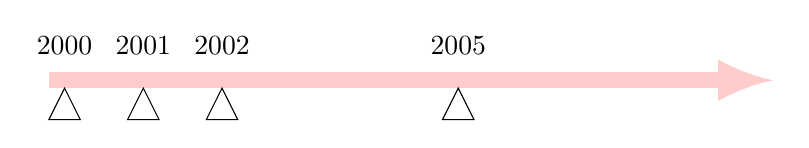
\begin{tikzpicture}
		\draw[line width=2mm,-latex,red!20] (-0.2,0) -- (9,0);
		\foreach \X [evaluate=\X as \Y using int(\X-2000),count=\Z] in {2000,2001,2002,2005}
		{
			\draw[highlight on=<\Z>] ({\Y-0.2},-0.5) -- ({\Y+0.2},-0.5) -- (\Y,-0.1) -- cycle;
			\node[anchor=south,highlight on=<\Z>,fill=white] at (\Y,0.2) {\X};
		}
	\end{tikzpicture}
	\begin{multicols}{2}
		\begin{itemize}
			\item<1-> November 2000: marmots start hibernating
			\item<2-> August 2001: marmots eat
			\item<2-> Semptember 2001: marmots eat
			\item<3-> July 2002: marmots eat
			\item<4-> May 2005: marmots awake from hibernation
			\item<4-> November 2005: marmots start hibernating again
		\end{itemize}
	\end{multicols}
\end{frame}
\end{document}


%%%%%%%%%%%%%%%%%%%%%%%%%%%%%%%%%%%%%%%%%%%%%%%%%%%%%%%%%%%%%%%%%%%%%%%%%%%%%%%%%%%%%%%%%%%%%%%%%%%%%%%%%%%%%%%%%%%%%%%%%%%%%%%%%%%%%%%%%%%%%%%%%%%%%%%%%%
